\documentclass[aspectratio=169]{beamer}
\usetheme{Madrid}
\usecolortheme{default}

% UTF-8 Hungarian charset support
\usepackage[utf8]{inputenc}
\usepackage[T1]{fontenc}
\usepackage[hungarian]{babel}
\usepackage{xcolor}


% Modern color scheme
\definecolor{primaryblue}{RGB}{41, 128, 185}
\definecolor{darkblue}{RGB}{52, 73, 94}
\definecolor{lightgray}{RGB}{236, 240, 241}
\definecolor{darkgray}{RGB}{52, 73, 94}
\definecolor{accent}{RGB}{231, 76, 60}
\definecolor{success}{RGB}{46, 204, 113}
\definecolor{warning}{RGB}{241, 196, 15}

% Set theme colors
\setbeamercolor{structure}{fg=primaryblue}
\setbeamercolor{palette primary}{bg=primaryblue,fg=white}
\setbeamercolor{palette secondary}{bg=darkblue,fg=white}
\setbeamercolor{palette tertiary}{bg=lightgray,fg=darkgray}
\setbeamercolor{palette quaternary}{bg=darkgray,fg=white}
\setbeamercolor{frametitle}{bg=primaryblue,fg=white}
\setbeamercolor{title}{fg=darkblue}
\setbeamercolor{block title}{bg=primaryblue,fg=white}
\setbeamercolor{block body}{bg=lightgray,fg=darkgray}
\setbeamercolor{block title alerted}{bg=accent,fg=white}
\setbeamercolor{block body alerted}{bg=accent!10,fg=darkgray}

% Remove navigation symbols
\setbeamertemplate{navigation symbols}{}

% Modern frame title
\setbeamertemplate{frametitle}{
    \begin{beamercolorbox}[wd=\paperwidth,ht=2.5ex,dp=1ex,leftskip=1em,rightskip=1em]{frametitle}
        \usebeamerfont{frametitle}\insertframetitle
    \end{beamercolorbox}
}

% Modern itemize
\setbeamertemplate{itemize items}[circle]
\setbeamercolor{itemize item}{fg=primaryblue}
\setbeamercolor{itemize subitem}{fg=darkblue}
\setbeamercolor{enumerate item}{fg=primaryblue}

\usepackage{listings}
\usepackage{graphicx}
\usepackage{tikz}
\usepackage{amsmath}
\usepackage{amssymb}
\usepackage[ruled,vlined]{algorithm2e}


\usetikzlibrary{shapes,arrows,positioning,calc}

\lstset{
  language=Python,
  basicstyle=\ttfamily\scriptsize,
  keywordstyle=\color{primaryblue}\bfseries,
  commentstyle=\color{success}\itshape,
  stringstyle=\color{accent},
  showstringspaces=false,
  frame=single,
  frameround=tttt,
  rulecolor=\color{lightgray},
  backgroundcolor=\color{lightgray},
  breaklines=true,
  numbers=left,
  numberstyle=\tiny\color{darkgray},
  stepnumber=1,
  numbersep=5pt,
  tabsize=2,
  columns=flexible,
  keepspaces=true,
}

\title{\Huge{HMSSQL}}
\author{Brustur-Buksa Beatrice, Dégi Nándor, Erdei Kristóf, Komjátszegi-Fábián Hunor}
\date{\today}

% Modern title page
\setbeamertemplate{title page}{
    \begin{center}
        \vspace{1cm}
        {\usebeamerfont{title}\usebeamercolor[fg]{title}\inserttitle\par}
        \vspace{0.5cm}
        {\usebeamerfont{author}\insertauthor\par}
        \vspace{0.3cm}
        {\usebeamerfont{date}\insertdate\par}
    \end{center}
}

\begin{document}

\frame{\titlepage}

\begin{frame}{Tartalom}
\tableofcontents[hideallsubsections]
\end{frame}

\section{Bevezetés és Rendszer Áttekintés}

\begin{frame}{Mi a HMSSQL?}
\begin{columns}
\begin{column}{0.6\textwidth}
\begin{itemize}
    \item \textbf{Kliens-Szerver Architektúra} socket-alapú kommunikációval
    \item \textbf{Cython-optimalizált B+ Fa} indexelés hatékony adatlekérdezéshez
    \item \textbf{Több Kliensfelület}: CLI, GUI (JavaFX)
    \item \textbf{Buffer Pool Menedzsment} hibrid LRU/LFU stratégiával
\end{itemize}
\end{column}
\begin{column}{0.35\textwidth}
\begin{alertblock}{Fő Innováció}
Cython-optimalizált B+ fa cursor-alapú paginálással és hibrid cache stratégiával a \textbf{10k+ rekord} hatékony kezeléséhez.
\end{alertblock}
\end{column}
\end{columns}
\end{frame}

\begin{frame}{Rendszer Architektúra Áttekintés}
\begin{center}
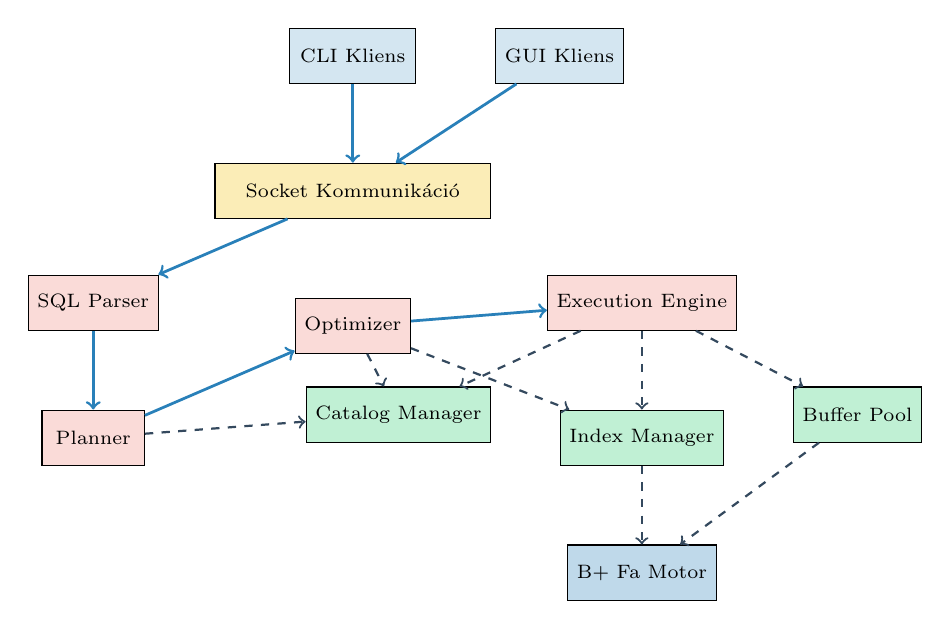
\begin{tikzpicture}[node distance=1cm, every node/.style={font=\scriptsize}]
    % Client Layer
    \node[rectangle, draw, fill=primaryblue!20, minimum width=1.6cm, minimum height=0.7cm] (cli) {CLI Kliens};
    \node[rectangle, draw, fill=primaryblue!20, minimum width=1.6cm, minimum height=0.7cm, right=of cli] (gui) {GUI Kliens};
    
    % Communication Layer
    \node[rectangle, draw, fill=warning!30, minimum width=3.5cm, minimum height=0.7cm, below=of cli] (comm) {Socket Kommunikáció};
    
    % Processing Pipeline (CORRECTED ORDER)
    \node[rectangle, draw, fill=accent!20, minimum width=1.3cm, minimum height=0.7cm, below left=of comm] (parser) {SQL Parser};
    \node[rectangle, draw, fill=accent!20, minimum width=1.3cm, minimum height=0.7cm, below=of parser] (planner) {Planner};
    \node[rectangle, draw, fill=accent!20, minimum width=1.3cm, minimum height=0.7cm, below=of comm] (optimizer) {Optimizer};
    \node[rectangle, draw, fill=accent!20, minimum width=1.3cm, minimum height=0.7cm, below right=of comm] (engine) {Execution Engine};
    
    % Storage Layer
    \node[rectangle, draw, fill=success!30, minimum width=1.3cm, minimum height=0.7cm, below left=of engine] (catalog) {Catalog Manager};
    \node[rectangle, draw, fill=success!30, minimum width=1.3cm, minimum height=0.7cm, below=of engine] (index) {Index Manager};
    \node[rectangle, draw, fill=success!30, minimum width=1.3cm, minimum height=0.7cm, below right=of engine] (buffer) {Buffer Pool};
    \node[rectangle, draw, fill=primaryblue!30, minimum width=1.3cm, minimum height=0.7cm, below=of index] (bptree) {B+ Fa Motor};
    
    % Main Pipeline Flow
    \draw[->, line width=1pt, color=primaryblue] (cli) -- (comm);
    \draw[->, line width=1pt, color=primaryblue] (gui) -- (comm);
    \draw[->, line width=1pt, color=primaryblue] (comm) -- (parser);
    \draw[->, line width=1pt, color=primaryblue] (parser) -- (planner);
    \draw[->, line width=1pt, color=primaryblue] (planner) -- (optimizer);
    \draw[->, line width=1pt, color=primaryblue] (optimizer) -- (engine);
    
    % Supporting Component Access
    \draw[->, line width=0.8pt, color=darkgray, dashed] (planner) -- (catalog);
    \draw[->, line width=0.8pt, color=darkgray, dashed] (optimizer) -- (catalog);
    \draw[->, line width=0.8pt, color=darkgray, dashed] (optimizer) -- (index);
    \draw[->, line width=0.8pt, color=darkgray, dashed] (engine) -- (catalog);
    \draw[->, line width=0.8pt, color=darkgray, dashed] (engine) -- (index);
    \draw[->, line width=0.8pt, color=darkgray, dashed] (engine) -- (buffer);
    \draw[->, line width=0.8pt, color=darkgray, dashed] (index) -- (bptree);
    \draw[->, line width=0.8pt, color=darkgray, dashed] (buffer) -- (bptree);
\end{tikzpicture}
\end{center}
\end{frame}

\section{B+ Fa Implementáció és Optimalizálás}

\begin{frame}{Cython-optimalizált B+ Fa}
\begin{block}{Miért Cython Optimalizálás?}
\begin{itemize}
    \item \textbf{C-szintű teljesítmény}: Közvetlen memóriakezelés és mutatók
    \item \textbf{Cache-barát}: Szekvenciális memória hozzáférés levelekben
    \item \textbf{Csökkentett Python overhead}: Kritikus útvonalak C-ben
    \item \textbf{SIMD optimalizálható}: Bináris keresés vektorizálással
\end{itemize}
\end{block}

\begin{block}{B+ Fa Implementációs Részletek}
\begin{itemize}
    \item \textbf{Levél csomópontok összekapcsolása}: \texttt{next\_leaf} mutatókkal
    \item \textbf{Értéktároló}: Külön \texttt{value\_store} ValueHoder osztály
\end{itemize}
\end{block}
\end{frame}

\begin{frame}[fragile]{Ismétlés}]
\begin{center}
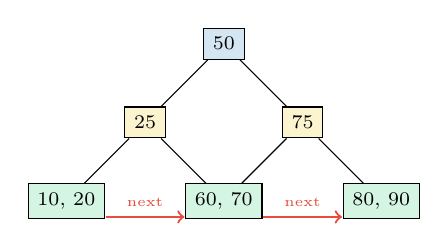
\begin{tikzpicture}[level distance=1cm, sibling distance=2cm, every node/.style={font=\scriptsize}]
    \node[rectangle, draw, fill=primaryblue!20] {50}
        child {
            node[rectangle, draw, fill=warning!20] {25}
            child {node[rectangle, draw, fill=success!20] {10, 20}}
            child {node[rectangle, draw, fill=success!20] {30, 40}}
        }
        child {
            node[rectangle, draw, fill=warning!20] {75}
            child {node[rectangle, draw, fill=success!20] {60, 70}}
            child {node[rectangle, draw, fill=success!20] {80, 90}}
        };
    
    % Leaf links with labels
    \draw[->, thick, color=accent] (-1.5,-2.2) -- (-0.5,-2.2) node[midway, above] {\tiny next};
    \draw[->, thick, color=accent] (0.5,-2.2) -- (1.5,-2.2) node[midway, above] {\tiny next};
\end{tikzpicture}
\end{center}

\begin{block}{Komplexitás Analízis}
\begin{align}
\text{Tree Traversal} &= O(\log_m n) \\
\text{Cursor Iteration} &= O(k) \text{ ahol } k = \text{eredmény méret} \\
\text{Space Complexity} &= O(1) \text{ további memória}
\end{align}
\end{block}
\end{frame}

\begin{frame}[fragile]{Range Query Algoritmus Specifikáció}
\begin{lstlisting}[language=Python]
def range_query(self, start_key, end_key):
    current_leaf = self._find_leaf_node(start_key)
    results = []
    while current_leaf is not None:
        for i, key in enumerate(current_leaf.keys):
            if key > end_key:
                return results
            if key >= start_key:
                value = self.value_store.get(key)
                if value is not None:
                    results.append((key, value))
        current_leaf = current_leaf.next_leaf
    return results

def _find_leaf_node(self, key):
    node = self.root
    while not node.is_leaf:
        i = 0
        while i < len(node.keys) and key > node.keys[i]:
            i += 1
        node = node.children[i]
    return node
\end{lstlisting}

\begin{alertblock}{Kritikus Tulajdonság}
\textbf{Early Termination}: Amikor \texttt{key > end\_key}, a keresés azonnal befejeződik, mivel a levelek rendezettek.
\end{alertblock}
\end{frame}

\section{Buffer Pool Menedzsment}

\begin{frame}[fragile]{Hibrid Cache Kiszorítási}
\begin{block}{Matematikai Modell}
Hibrid pontszám minden \texttt{page\_id}-hez:
\begin{align}
\text{Score}(p) &= w_f \cdot \text{Frequency}(p) + w_t \cdot \text{Recency}(p) \\
\text{Frequency}(p) &= \text{access\_count}(p) \\
\text{Recency}(p) &= \text{current\_time} - \text{last\_access}(p) \\
w_f + w_t &= 1.0, \quad w_f = 0.7, w_t = 0.3
\end{align}
\end{block}
\end{frame}

\begin{frame}[fragile]{Buffer Pool Kiszorítási Algoritmus}
\begin{lstlisting}[language=Python]
def _evict_page(self):
    if self.strategy == CacheStrategy.HYBRID:
        current_time = time.time()
        
        victim_id = min(
            self.pages.keys(),
            key=lambda k: (
                self.access_counts[k] * 0.7 +                    
                (current_time - self.last_access_time[k]) * 0.3  
            )
        )
    
    if victim_id in self.dirty_pages:
        self._write_back(victim_id, self.pages[victim_id])
        self.dirty_pages.remove(victim_id)
    
    del self.pages[victim_id]
    del self.last_access_time[victim_id]
    del self.access_counts[victim_id]
\end{lstlisting}

\begin{block}{Kiszorítási Hatékonyság}
Hibrid stratégia \textbf{optimális egyensúlyt} teremt a gyakran és nemrég használt oldalak között.
\end{block}
\end{frame}

\section{Index Manager és Optimalizálás}

\begin{frame}{Index Manager Architektúra}
\begin{block}{Index Típusok és Kezelés}
\begin{itemize}
    \item \textbf{Unclustered indexek}: Külön \texttt{.idx} fájlokban
    \item \textbf{Összetett indexek}: Többoszlopos kulcsok támogatása
    \item \textbf{Index cache}: Memóriában tartott gyakran használt indexek
    \item \textbf{Automatikus újraépítés}: Sérült indexek helyreállítása
\end{itemize}
\end{block}

\begin{block}{Index Fájl Struktúra}
\begin{itemize}
    \item \textbf{Fájlnév}: \texttt{db\_table\_column.idx}
    \item \textbf{Szerializálás}: Pickle-alapú B+ fa perzisztencia
    \item \textbf{Metaadatok}: Index konfiguráció és statisztikák
    \item \textbf{Verziószám}: Cache invalidáció támogatás
\end{itemize}
\end{block}
\end{frame}

\begin{frame}[fragile]{Index Építés és Cache Kezelés Algoritmus}
\begin{lstlisting}[language=Python]
def build_index(self, table_name, index_name, column, is_unique=False):
    full_name = f"{table_name}.{index_name}"
    
    if full_name in self.indexes_cache:2
        return self.indexes_cache[full_name]
    
    index_file = f"{self.data_dir}/{self.db_name}_{table_name}_{column}.idx"
    
    if os.path.exists(index_file):
        with open(index_file, 'rb') as f:
            index = pickle.load(f)
    else:
        index = BPlusTree(order=50)
        records = self.catalog_manager.get_all_records(table_name)
        
        for record_id, record in enumerate(records):
            if column in record:
                key = record[column]
                existing = index.search(key)
                
                if is_unique:
                    index.insert(key, record_id)
                elif existing is None:
                    index.insert(key, [record_id])
                else:
                    value = existing if isinstance(existing, list) else [existing]
                    value.append(record_id)
                    index.insert(key, value)
        
        with open(index_file, 'wb') as f:
            pickle.dump(index, f)
    
    self.indexes_cache[full_name] = index
    return index
\end{lstlisting}
\end{frame}

\section{Lekérdezés Optimalizálás}

\section{Végrehajtási Pipeline}

\begin{frame}{Végrehajtó Motor Optimalizálás}
\begin{block}{Pipeline Komponensek}
\begin{itemize}
    \item \textbf{Select Executor}: Index-tudatos lekérdezés végrehajtás
    \item \textbf{Join Executor}: Algoritmus-specifikus optimalizálás
    \item \textbf{Aggregate Executor}: Memóriahatékony csoportosítás
    \item \textbf{DML Executor}: Batch művelet támogatás
\end{itemize}
\end{block}

\begin{block}{Memória Kezelés Nagy Adathalmazoknál}
\begin{itemize}
    \item \textbf{Streaming execution}: Nem tölti be az összes rekordot
    \item \textbf{Buffer pool integration}: Oldal-alapú hozzáférés
    \item \textbf{Cursor-based iteration}: Inkrementális eredmény generálás
    \item \textbf{Early termination}: LIMIT-eknél korai kilépés
\end{itemize}
\end{block}
\end{frame}

\begin{frame}[c]
\begin{center}
{\Huge Köszönjük a figyelmet!}

\vspace{0.5cm}

\includegraphics[width=0.3\textwidth]{meme} 
\end{center}
\end{frame}

\end{document}